\documentclass[compress, red]{beamer}
\mode<presentation>
\usetheme{Warsaw}
\usecolortheme{lily}
\useoutertheme[subsection=false]{smoothbars}
\useinnertheme{rectangles}

\title{Totally Bounded, Compact and Complete Metric Spaces}
\author{Anmol Bhullar}
\institute{MATC27}
\date{December 2017}

\begin{document}
    \frame{\titlepage}

    \begin{frame}
        \frametitle{Motivation}
        Consider $(-1,1)$ as a topological space.
        \begin{itemize}
            \item<1-> We might be tempted to say this is bounded but we have no machinery to do so.
            \item<2-> Enter Metric Spaces
            \item<3-> Not all metric spaces are bounded but it would be interesting some conditions that guarantee the bounded property
            \item<4-> Intuitively, we want the existence of a \textit{real} number $r$ such that the distance between any two points in 
                the space is less than $r$.
        \end{itemize}
    \end{frame}

    \begin{frame}
        \frametitle{What do we mean by a "Bounded Space"?}
        \begin{definition}
            A metric space $(X,d)$ is \alert{bounded} if there exists some number $r\in\mathbb{R}$ such that $d(x,y)\leq r$ for all $x,y\in X$. We might
            say $r$ is \textit{upper bound}, and the smallest of all such $r$'s is said to be the \textit{diameter} of the set $X$ (in the context 
            of $d$).
        \end{definition}
        \begin{itemize}
            \item<1-> Homeomorphic to another bounded space?
            \item<2-> Subspace of a bounded space?
            \item<3-> Product of a bounded space?
            \item<4-> Compactness?
        \end{itemize}
    \end{frame}

    \begin{frame}
        \frametitle{When is a metric space bounded?}
        \begin{theorem}
            If $f: X \to Y$ is a homeomorphism and $X$ is bounded, $Y$ is not necessairly bounded. Subspace of a bounded metric is bounded.
            (At most) countable products of bounded metric spaces are bounded.
        \end{theorem}
        Proof:
        \begin{itemize}
            \item<1-> $(-1,1)\cong \mathbb{R}$
            \item<2-> Recall the subspace is given the submetric. So if $Y$ is a subspace of $X$ which is a bounded space, then
                $d_Y(x,y) = d_X(x,y) < r$.
        \end{itemize}
    \end{frame}

    \begin{frame}{The Product Metric}
        \begin{definition}[The product metric]
            Let $(X_1,d_1),\hdots,(X_n,d_n),\hdots$ be a sequence of metric spaces. 
            For a finite product, we have $d((x_1,\hdots,x_n),(y_1,\hdots,y_n)) = $
            \[ \sqrt{d_1(x_1,y_1)^2 + d_2(x_2,y_2)^2 + \hdots + d_n(x_n,y_n)^2} \]
            where $d$ is a metric on $X_1\times\hdots\times X_n$. For an infinite product on $\Pi_{k=1}^{\infty} X_k$, we have:
            \[ d(x,y) = \sum_{k=1}^{\infty} \frac{1}{2^k} \cdot \frac{d_k(x_k,y_k)}{1+d_k(x_k,y_k)} \]
        \end{definition}
    \end{frame}

    \begin{frame}{Proof (continued)}
        Main Idea:
        \[ d(x,y) = \sum_{k=1}^{\infty} \frac{1}{2^k}\frac{d_k(x_k,y_k)}{1+d_k(x_k,y_k)} < \sum_{i=1}^{\infty} \frac{1}{2^k}\frac{r_k}{1+r_k}\in
            \mathbb{R}\]
        or
        \[ d(x,y) = \big{(}\sum_{k=1}^n d_k(x_k,y_k)^2\big{)}^{\frac{1}{2}} < \big{(}\sum_{k=1}^n r_k^2\big{)}^{\frac{1}{2}} \in \mathbb{R} \]
        No generalization possible for uncountable products of metric spaces
    \end{frame}

    \begin{frame}{Compactness}
        We have already seen that every compact metric space is bounded.\\
        
        Let us recall the definition of compactness in a topological space.
        \begin{definition}[Open Cover Definition]
            Let $X$ be a topological space. $X$ is compact iff each of its open covers admit a finite subcover.
        \end{definition}
        \begin{itemize}
            \item<2-> We might want to re-write this definition to emphasize the \textit{boundedness} property. 
            \item<3-> This is the motivation for our next definition
        \end{itemize}
    \end{frame}

    \begin{frame}
        \frametitle{Motivation: Totally Bounded}
        Consider:
        \begin{itemize}
            \item<2-> Let $X$ be a compact metrizable space. Choose an open cover which is a collection of open balls of at most diameter $\epsilon$.
            \item<3-> Through compactness, we can find a \textit{finite} collection of open balls which are at most diameter $\epsilon$.
            \item<4-> We can do this for all $\epsilon>0$
            \item<5-> Therefore, for all $\epsilon>0$, we can find a finite collection of open balls at most diameter $\epsilon$ which cover $X$.
            \item<6-> Call $X$ \alert{totally bounded}
        \end{itemize}
    \end{frame}

    \begin{frame}
        \frametitle{Totally Bounded}
        \begin{definition}
            A metric space $(X,d)$ is \alert{totally bounded} if and only if for every real number $\epsilon>0$, there exists a finite collection of
            open balls in $X$ of radius $\epsilon$ whose union contains $X$.
        \end{definition}
        Now, we check if \textit{at least} total bounded $\implies$ bounded. If this is not true, we have a big problem with out definition :(
    \end{frame}

    \begin{frame}
        \frametitle{Relationship between bounded and totally bounded}
        \begin{theorem}[Totally Bounded $\implies$ Bounded]
            Let $X$ be a totally bounded metric space. We show that $X$ is bounded and show the converse is not necessairly true.
        \end{theorem}
        Proof:
        \begin{itemize}
            \item<2-> Choose $\epsilon>0$, and choose the associated finite collection of open balls which cover $X$. (denote by $\mathcal{B}$).
                Suppose these are centered at $x_0,x_1,\hdots,x_k\in X$.
            \item<3-> Show $d(x_i,x)$ is bounded and $d(x_j,y)$ is bounded.
            \item<4-> Use this to show $d(y,x)$ is bounded (triangle inequality)
        \end{itemize}
    \end{frame}

    \begin{frame}
        \frametitle{Proof continued}
        Now for a counterexample to show bounded $\implies$ totally bounded is not true!
        \begin{itemize}
            \item<2-> Think simple! What is simple? The discrete metric
            \item<3-> Let $|X| = \infty$. Equip this with the discrete metric $d$. This is bounded (why?)
            \item<4-> Can we cover this with a collection of open balls with diameter $\epsilon \leq 1$?
            \item<5-> Are we done the proof? No. Recall, we want to show the converse is not \alert{necessairly} true!
            \item<6-> Is $(-1,1)$ totally bounded? compact?
        \end{itemize}
    \end{frame}

    \begin{frame}
        \frametitle{Totally Bounded $\implies$ compact?}
        \begin{itemize}
            \item<2-> We've established that compact $\implies$ totally bounded
            \item<3-> We've also seen that totally bounded $\implies$ compact is not necessairly true.
            \item<4-> Is there some condition we can add to totally bounded to give us compactness? Hint: What went wrong in $(-1,1)$?
            \item<5-> Does it make more sense to want closedness or  completeness ?
        \end{itemize}
    \end{frame}

    \begin{frame}
        \frametitle{Complete Metric Spaces}
        \begin{definition}
            A sequence $\{x_n\}$ in a metric space $(X,d)$ is called a \alert{Cauchy sequence} iff for every $\epsilon>0$ there exists
            an integer $N$ such that $d(x_m,x_n)<\epsilon$ whenever $m,n>N$.
        \end{definition}
        Why Cauchy convergence and not the normal notion?
        \begin{example}
            Let $x_n := \frac{1}{n}$. The set $(x_n)$ has no limit point but we can still talk about its \alert{Cauchy} convergence
            with no reference to what it might converge to. 
        \end{example}
    \end{frame}

    \begin{frame}{Complete Metric Spaces (continued)}
        \begin{definition}
            A \alert{complete} metric space is a metric space in which every Cauchy sequence converges to some point \textit{in} the same space.
        \end{definition}
        \begin{itemize}
            \item<2-> Let's return to $(-1,1)$. This is not complete, but we can see that $[-1,1]$ is. How did I get to $[-1,1]$?
            \item<3-> Every compact metric space is complete (converse not true in general)
            \item<4-> Is this a topological property? (There $\exists$ a one line "proof" to this)
        \end{itemize}
    \end{frame}

    \begin{frame}
        \frametitle{Every compact metric space is complete}
        Recall:
            $x$ is a limit point of the set $A$, if every deleted neighbourhood $U$ of $x$ has a non-empty intersection with $A$.
        \begin{itemize}
            \item<2-> Recall a set is closed iff it contains all of its limit points. What might that say for the points that Cauchy sequences 
                converge to?
            \item<3-> Recall if a topological space is compact, and a subspace of it is closed, then...
            \item<4-> How might we choose a subspace to show that $X$ is compact?
            \item<5-> Don't forget the $\blacksquare$
        \end{itemize}
    \end{frame}

    \begin{frame}
        \frametitle{Totally Bounded + Complete $\implies$ Compact}
        \begin{proof}
            Let $X$ be a totally bounded and complete metric space where $d$ is our metric.
            \begin{itemize}
                \item<2-> Pick an open cover $\{\theta_{\alpha}\}$ and assume it has no finite subcover.
                \item<3-> Use the totally bounded condition and pick a collection of open balls of radius 1. One such ball is not covered by a
                    finite subcollection of $\{\theta_{\alpha}\}$. Pick such a ball $B_d(x_0,1)$.
                \item<4-> Repeat process so we get a sequence $x_n := x_i \in B(x_i,2^{-n})$. Note each $B(x_i,2^{-n})$ cannot be covered by
                    a finite subcollection of $\{\theta_{\alpha}\}$.
                \item<5-> $x\in\theta_{\alpha} \implies \exists r>0$ such that $B(x,r)\subseteq\theta_{\alpha}$. Show this covers infinite points
                    of $x_n$ which is a contradiction.
            \end{itemize}
        \end{proof}
    \end{frame}

    \begin{frame}
        \frametitle{Compact $\implies$ Complete + Totally Bounded}
        We have shown Compact $\implies$ Totally Bounded.\\
        We have shown Compact $\implies$ Complete.$\blacksquare$
    \end{frame}

    \begin{frame}
        \frametitle{A compact meme}
        \begin{figure}
            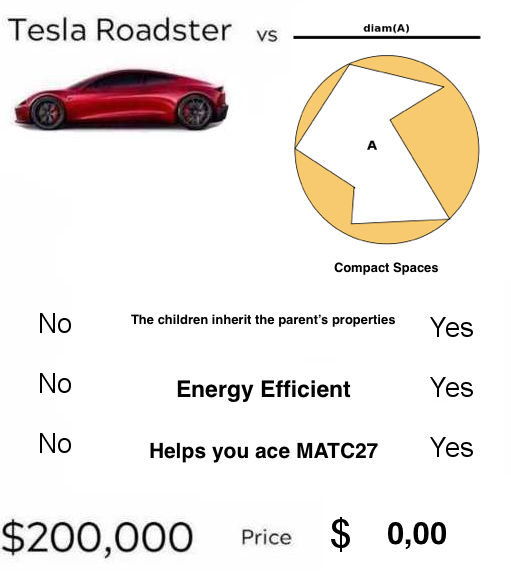
\includegraphics[scale=0.25]{meme}
        \end{figure}
    \end{frame}

\end{document}
